\chapter{Habitat of ice reservoirs}

\cleanchapterquote{Ice stupas offer a solution to the shortage of water all our mountain regions are
	facing.}{Pema Gyamtsho }{(Director General, International Center for Integrated Mountain Development)}

\ac{AIRs} cannot be built anywhere. They require favourable meteorological conditions, sufficient water supply,
and specific topography to amass a seasonal stock of ice. However, these three requirements are coupled and
exhibit drastic spatio-temporal variations. Therefore, generalising results from AIRs studied in this thesis to
obtain future volume estimates in new construction locations is plagued with uncertainty.

In this chapter, we leverage all our ice volume observations to disentagle the relationship between meteorology
and topography to provide first order estimates of interregional, intraregional and interannual ice volume
variations. 

\section{Interregional ice volume variability}

\ac{AIRs} built in the Himalayas and the Alps show drastic ice volume variations. Comparison of ice stupa volume
evolution show that the Indian structures grew four times larger than the Swiss ones (Fig. \ref{fig:2AIRs}). The
ice volume achieved after the accumulation period was much higher for the Indian ice stupa compared to the Swiss
ice stupas. The lower net radiation fluxes of the Indian location favored a faster thickness growth and the
spray radius of the Indian fountain produced a higher surface area compared to the Swiss counterparts (paper I).
These results indicate that the colder, drier and less cloudy meteorological characteristics of the Ladakh
region made it more suitable to build \ac{AIRs} compared to the Guttannen region. Therefore, arid and
glacial-fed mountain catchments for example, in Chile, Peru and Nepal are expected to be ideal locations to use
ice harvesting tools for seasonal water storage.

\section{Intraregional ice volume variability}

\begin{figure}
	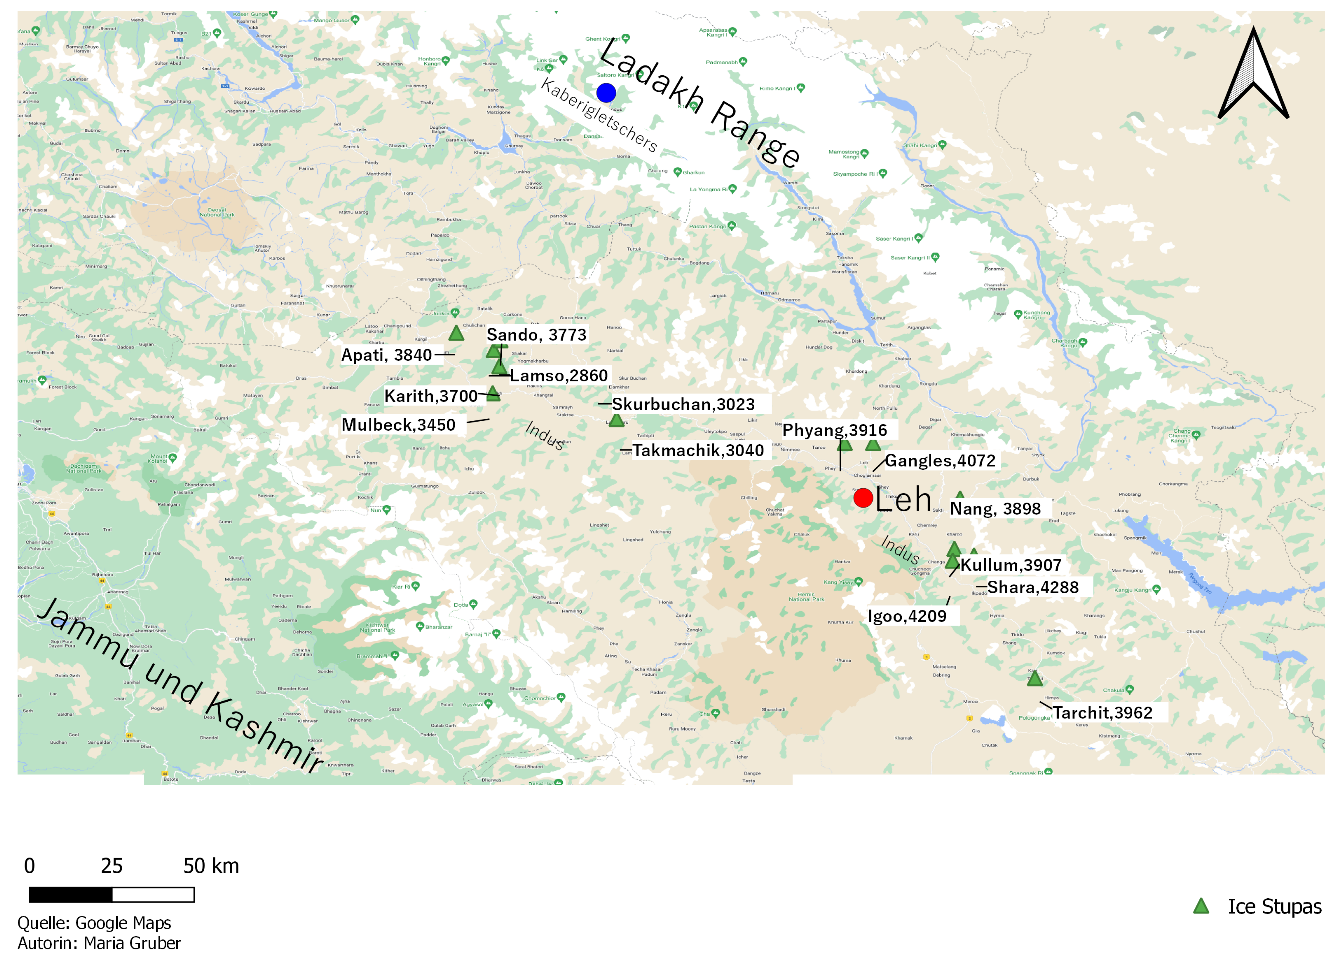
\includegraphics[width=\textwidth]{figs/ISC_villages}
	\caption{Villages of Ladakh where ice stupa volume observations are available. Adapted from \citet{mariagruberIceStupasLadakh2022}.}
	\label{fig:villages}
\end{figure}

We measured ice volumes in more than 14 villages in Ladakh (Fig. \ref{fig:villages}). Their volume variation
reveals a correlation with the altitude of the construction location (Fig. \ref{fig:altvsvol}). This correlation
indicates that elevation gain of 100 $m$ causes a corresponding ice volume gain of 1 million litres. However,
some locations with lower altitudes exhibit higher volumes compared to those with a higher altitude. This is due
to topographic effects of shadow valleys that reduce the sunshine hours of the location
\citep{mariagruberIceStupasLadakh2022}.

\begin{figure}
	\centering
	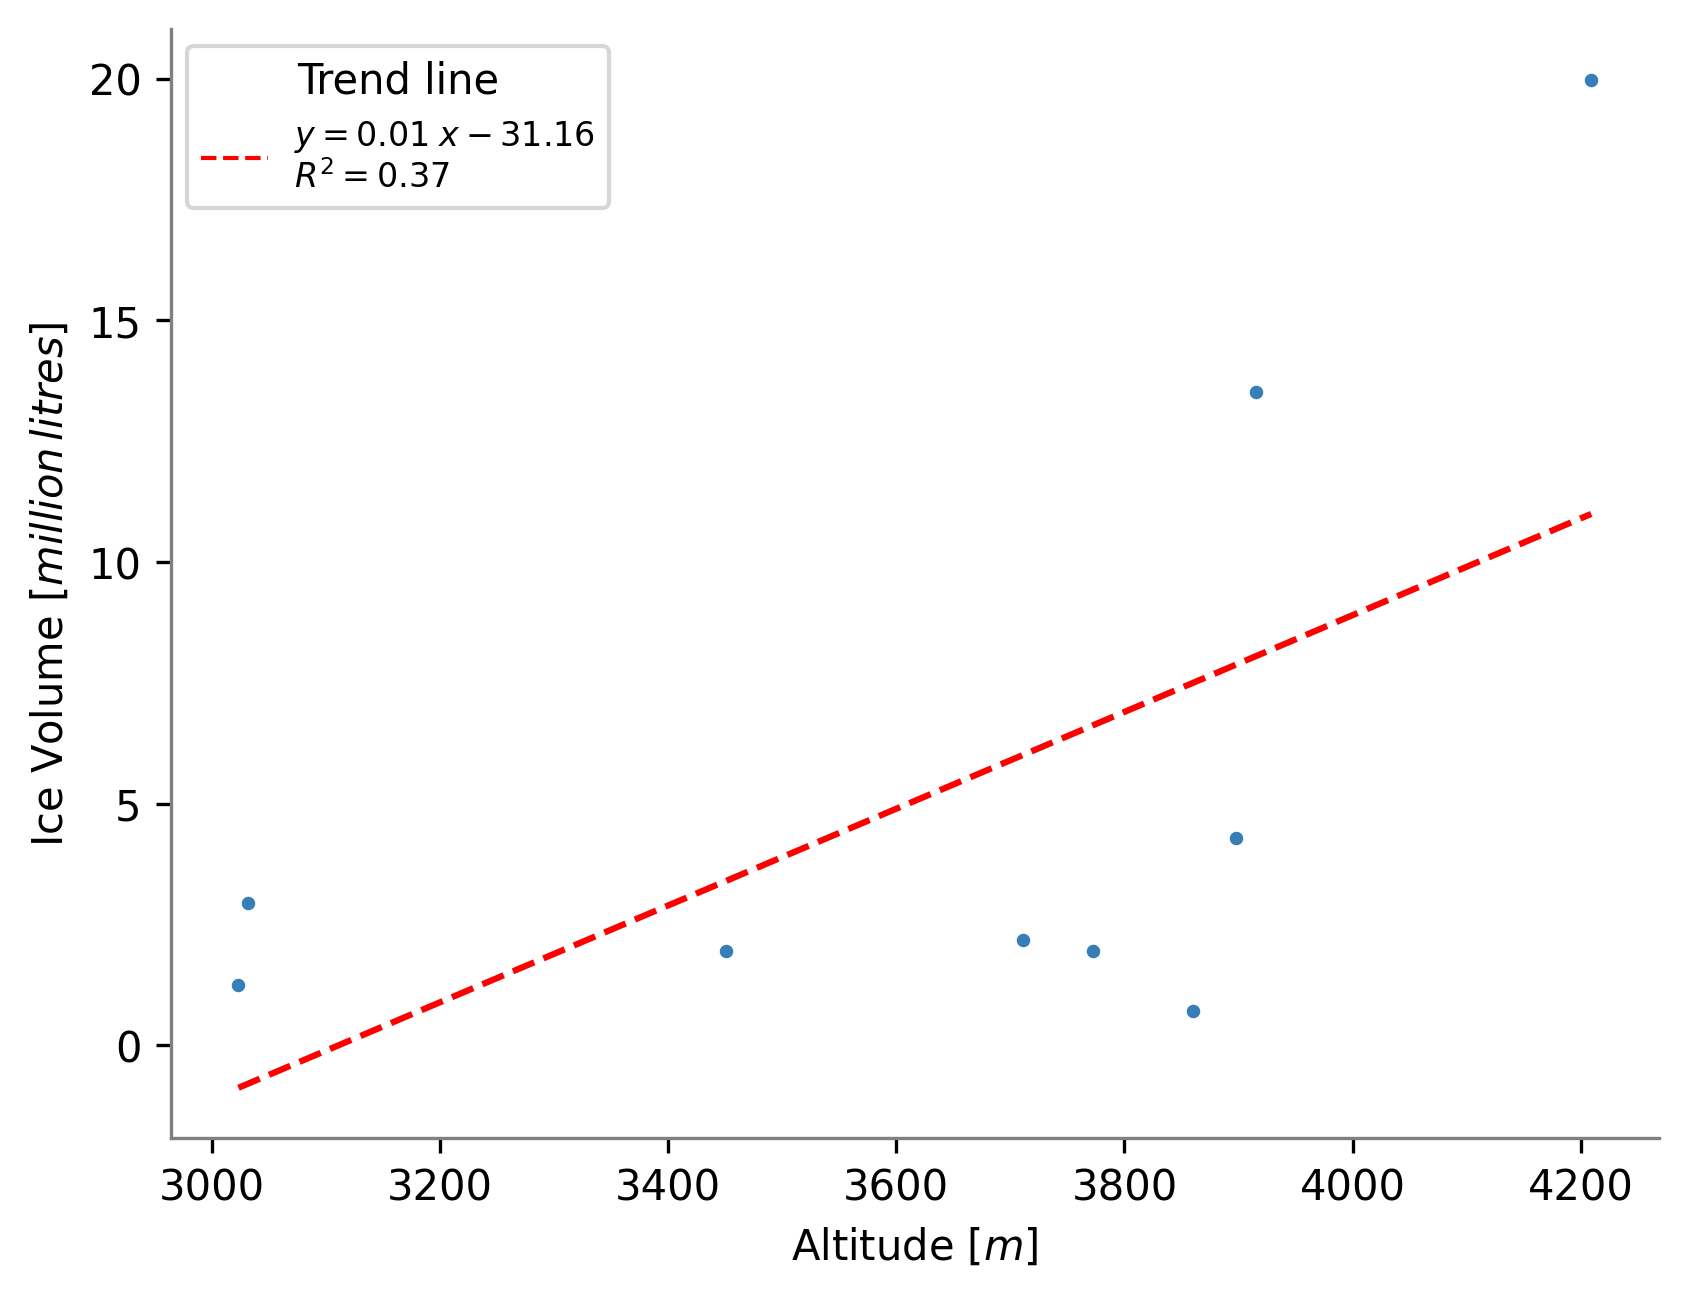
\includegraphics[width=\textwidth]{figs/altitudevsvolume.png}
	\caption{Relationship of measured ice volume (blue dots) with altitude of \ac{AIRs} built during winter of 2019-20 across
		different villages in Ladakh. Adapted from \citet{mariagruberIceStupasLadakh2022}.}
	\label{fig:altvsvol}
\end{figure}

Two ice stupas built in villages above 4200 m \ac{a.s.l.} (Shara and Igoo) have also been observed to last
beyond a summer melt season (Fig. \ref{fig:PIR}). However, such favourable meteorological conditions remain to
be discovered in the Swiss mountains. A possible way to study this question is to decrease the air temperature
Swiss ice stupas are exposed to uniformly (temperature change $\Delta T$). This will imply a stronger negative
sensible heat flux in summer, thus accelerating ice stupa growth and slowing down its decay. Such simulations
were produced using the Oerlemans model for an ice stupa grown in the Diavolezza site at an altitude of 2080 m
\ac{a.s.l.}. We found a break-even point for $\Delta T = -2 \degree C$ (Fig. \ref{fig:PIR_evolution}). For
larger negative values of $\Delta T$ the ice stupa does not disappear in summer and keeps growing from year to
year. For $\Delta T = -3 \degree C$, the maximum volume in the fifth year is about 4 times that in the first
year (Fig. \ref{fig:PIR_evolution}). Therefore, we hypothesize that ice stupas can last beyond a year even in
Switzerland if built in locations with an elevation above 2388 $m$ (based on a standard atmospheric lapse rate
of 0.0065 $\degree\,C\,m^{-1}$).

\begin{figure}
	\centering
	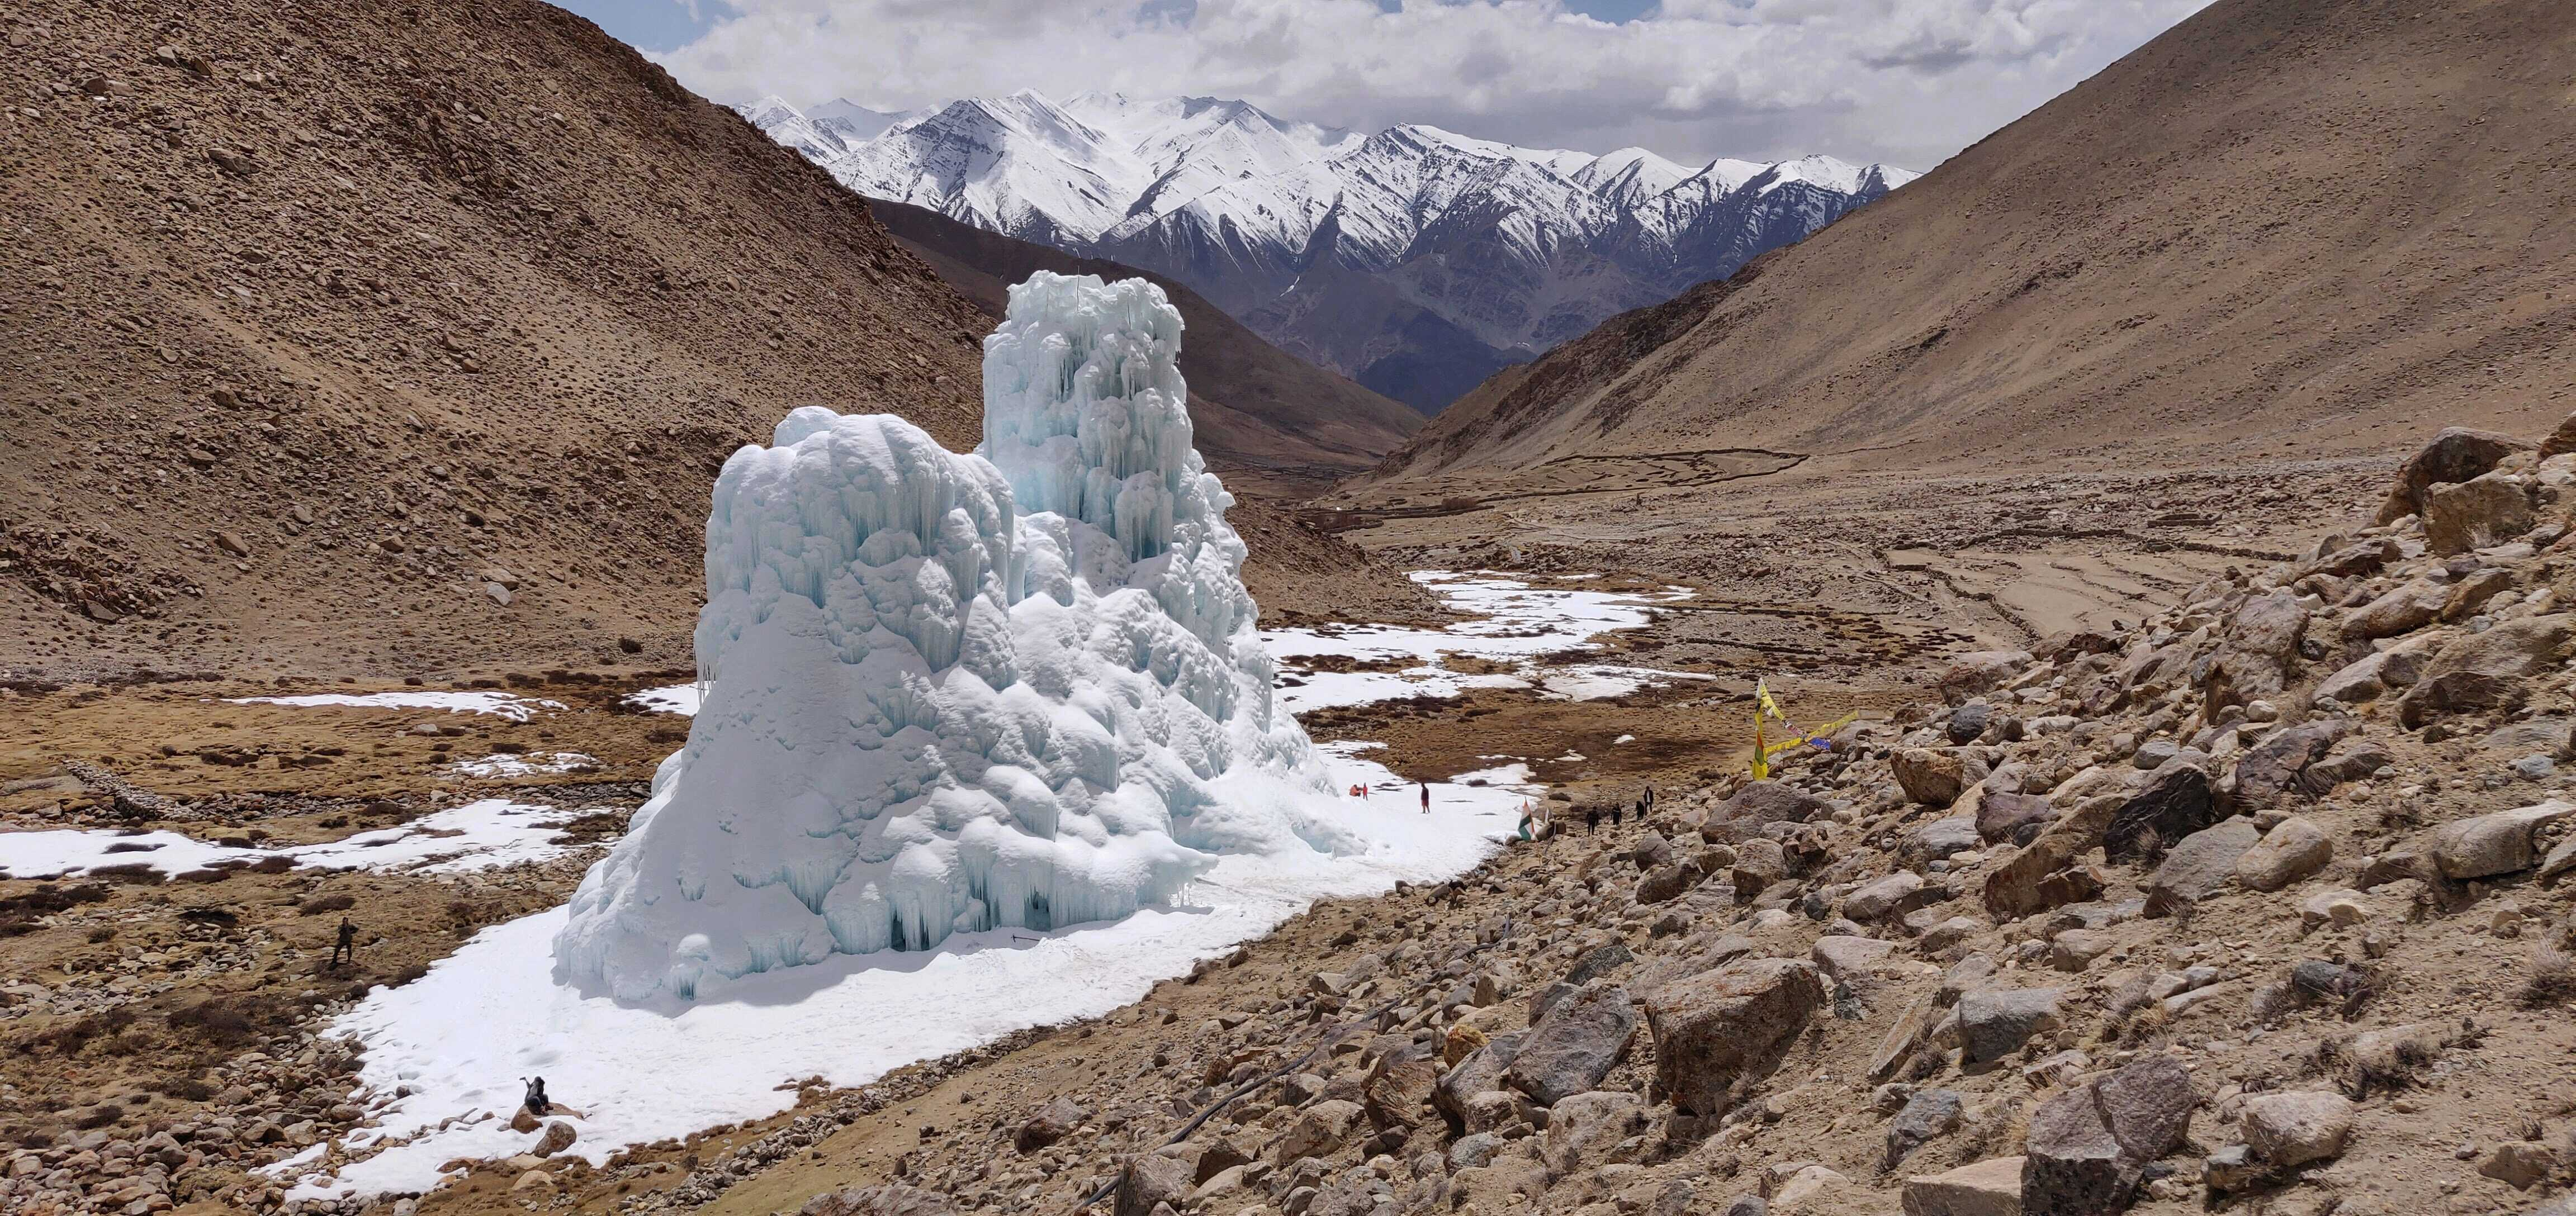
\includegraphics[width=\textwidth]{figs/PIR_example.jpg}

	\caption{Icestupa at Shara, Ladakh, built by local farmers in the winter of 2019-20, survived a full summer melt season and released
		around 8 million litres of water.}

	\label{fig:PIR}
\end{figure}

\begin{figure}
	\centering
	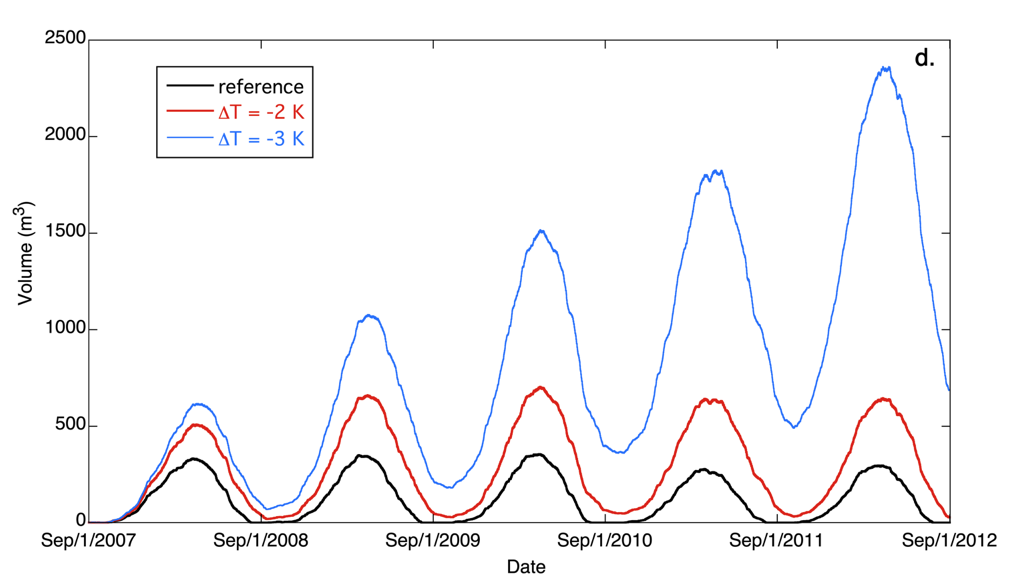
\includegraphics[width=\textwidth]{figs/PIR_evolution.png}
	\caption{The effect of a negative temperature perturbation. For $\Delta T = -3 \degree C$ the icestupa does
		not disappear anymore but is growing from year to year.}
	\label{fig:PIR_evolution}
\end{figure}


\section{Interannual ice volume variability}
\label{sec:interannual}

\begin{figure}
	\centering
	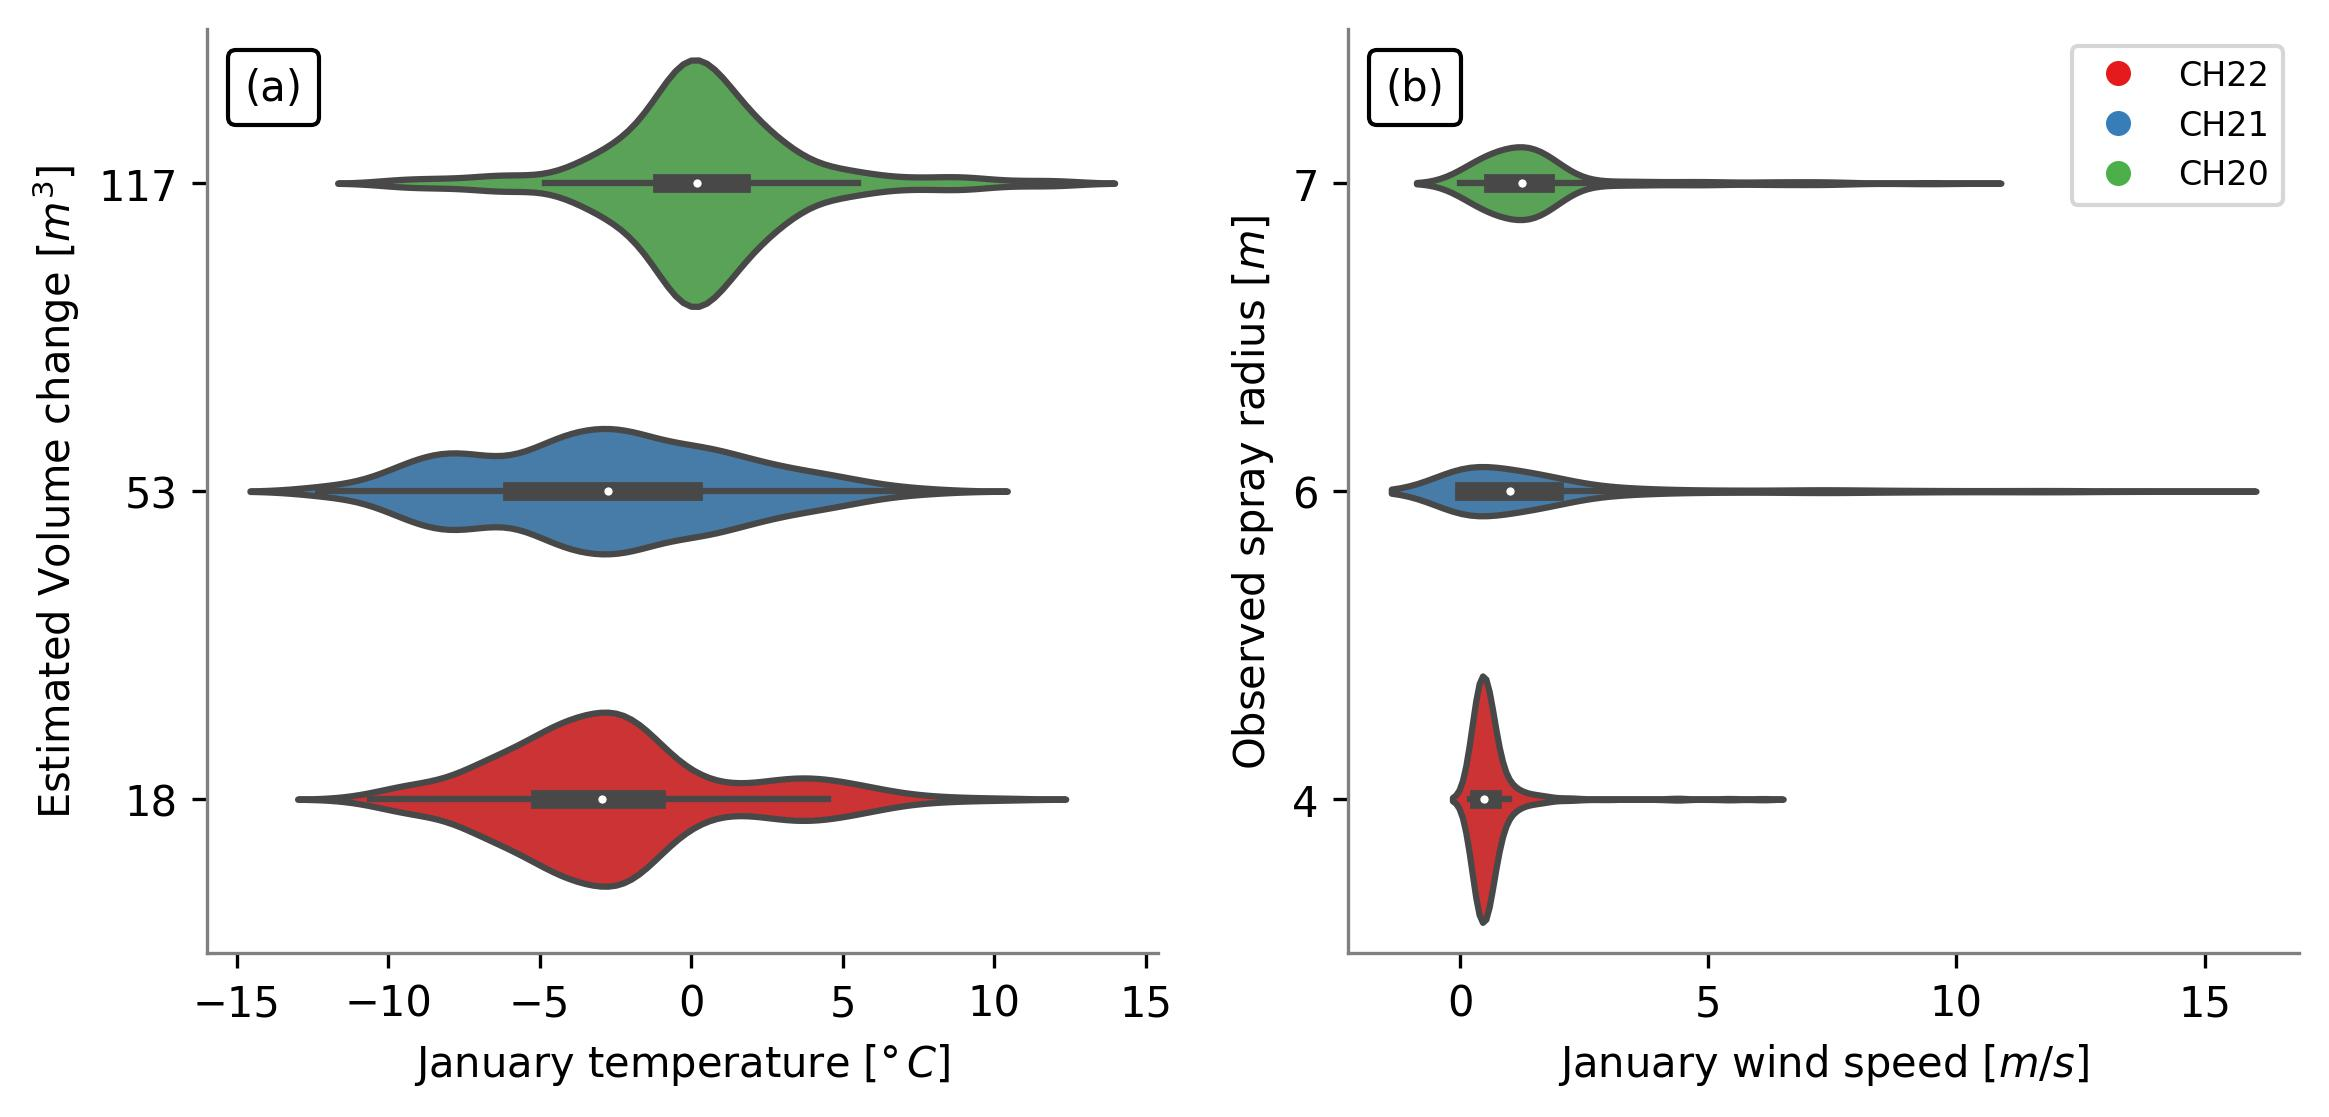
\includegraphics[width=\textwidth]{figs/CH_diffs.jpg}
	\caption{(a) Estimated volume change and temperature and (b) Observed spray radius and wind speed
		during January for \ac{AIRs} built across three winters. }
	\label{fig:CH_diffs}
\end{figure}

\ac{AIRs} built in Switzerland across three winters (CH20, CH21 and CH22) show a decreasing trend in their ice volume
changes for the month of January. Contrary to expectations, this decreasing trend was not caused by increasing
temperatures but rather by decreasing wind speeds (Fig. \ref{fig:CH_diffs}). A process-based analysis revealed
that wind driven redistribution of solid precipitation could explain these differences (paper II). The influence of this process on
the fountain spray radius managed to generate \ac{AIRs} six times bigger in spite of temperatures being 3 $\degree C$
warmer (Fig. \ref{fig:CH_diffs} (b)).



